%You can use any data modeling approach to describe the data aspects of "OBJECTS"
\section{PASS and Data modeling}
\label{sec:PassAndData}

PASS is predominantly a modeling language intended to describe processes. However, especially in the context of business processes, interaction with data-objects, often referred to as business objects, are necessary. PASS explicitly calls for modeling these aspects as was already mentioned in section \ref{sec:subjectInteraction} or more specific subsections \ref{sec:fullySpecifiedSubject} and \ref{sec:MessagePayload}.

\PASSModelElement{Subjects} as well as \PASSModelElement{Messages} are assumed to have an individual "data storage" capacity.  A Message Specification  \PASSModelElementObjectPropertie{contains [a] Payload Description} in form of a \textbf{Payload Data Object Definition}. A Subject simply \PASSModelElementObjectPropertie{has [a] Data Definition}. According the principle of subject-orientation, these data stores are \textbf{passive} and never do anything on their own, they simply "are there" or "exist". 

In principle, any means or technology to define data structures (\PASSModelElement{Data Object Definition}) and constraints upon them can be used for that purpose, as long as the intended recipient of the model is able to understand it. The technical precondition here is the existence of an exchange format for the data structure definitions that can be used to be stored with the PASS model. Examples are XML-Schema, RDF-Schema (RDFS), or OWL. Due to the model exchange standard for PASS itself being founded on OWL, using that language's means to define data types/classes and constraints upon them and directly integrating them into the model is a suitable approach.

The minimum capability to model the structure of Subjects Data Object Definitions and Message Payloads should be the ability to define the existence of data fields, as well as their data type, their order, and how often they occur in the data structure (e.g. single occurrence or multiple occurrence aka a list). Standard data types for the fields are what can typically be found in any data related descriptions means, e.g. data base query definitions via SQL that contain concepts like  integer and floating point numbers, boolean, string, and date/time. Beyond that, the ability to define further, complex data types/classes (\textbf{Data Type Definition}), comprised of other data objects, is expected to exists. Figure \ref{fig:examplePayloadDef} shows such a simple and generic definition approach.

\begin{figure*}[htbp]
	\centering
	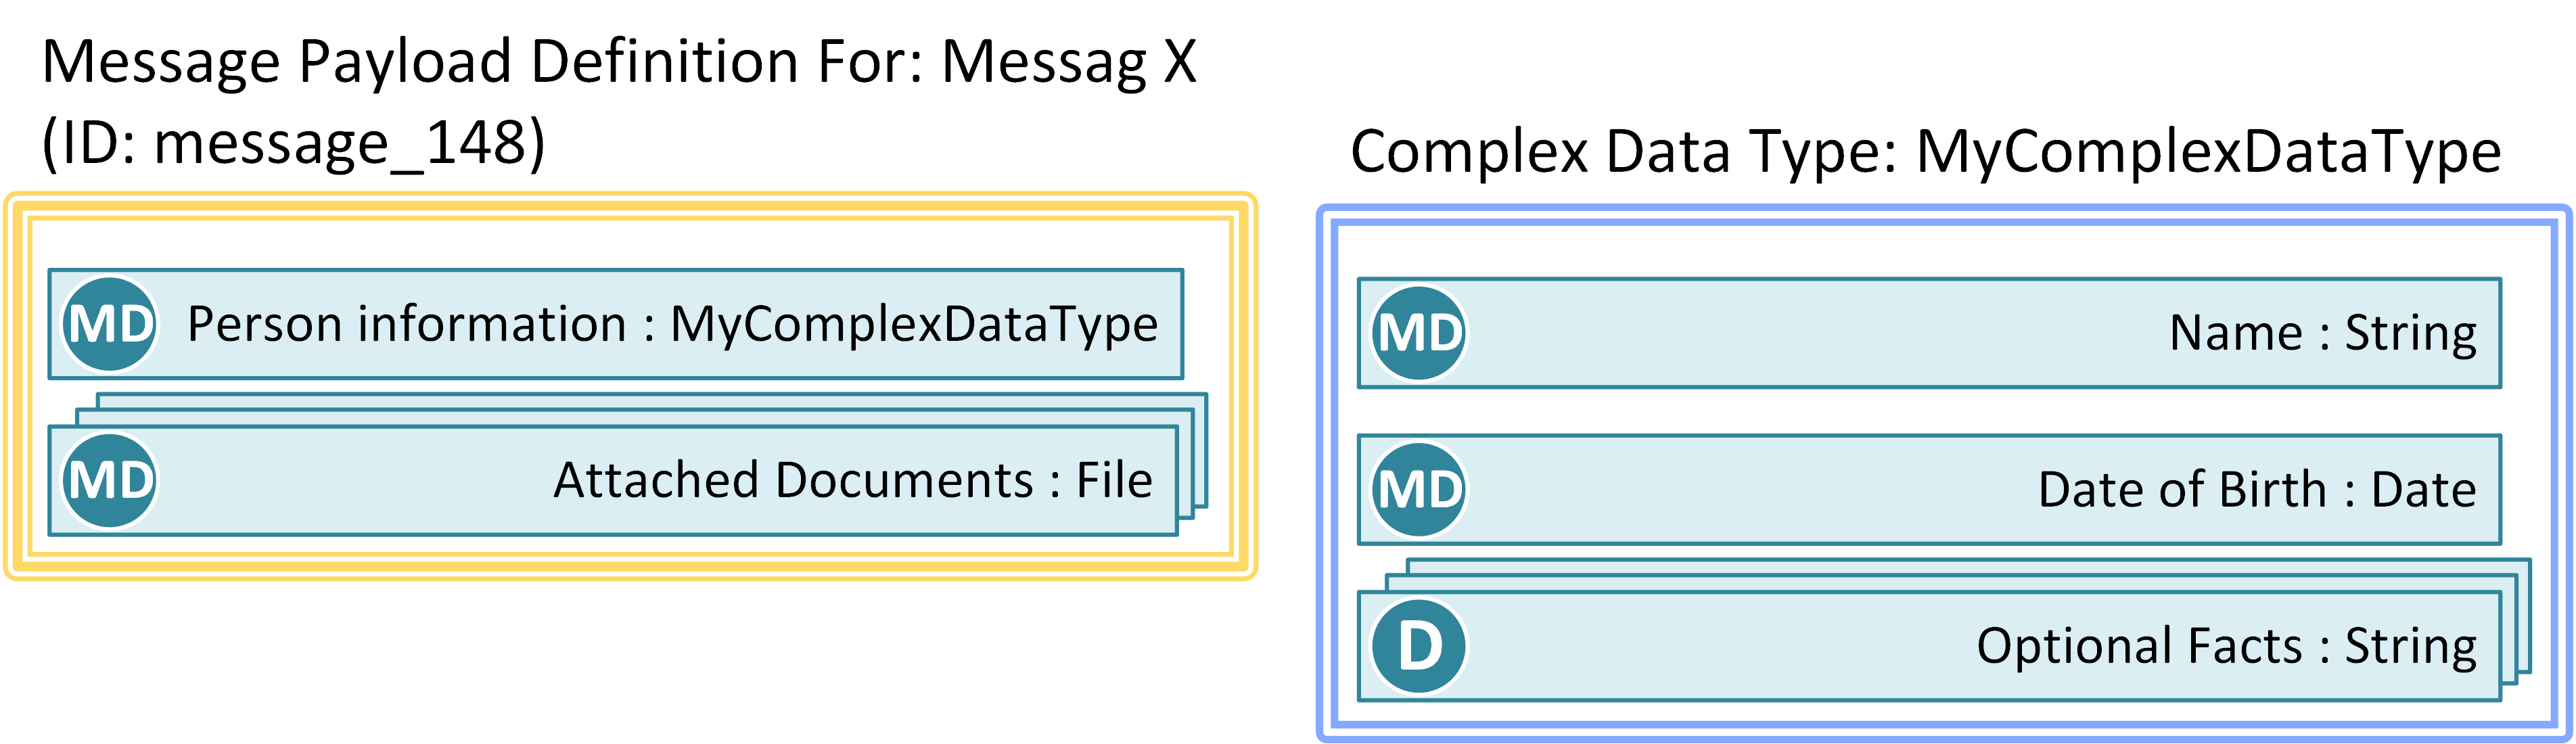
\includegraphics[width=14cm]{Figures/ExamplePayloadAndTypeDefinitions.png}
	\caption[Example for a generic Message Payload Definition with field names and data types, including the specification of a Custom Datatype]{Example for a generic Message Payload Definition with field names and data types, including the specification of a Custom Datatype}
	\label{fig:examplePayloadDef}
\end{figure*}

\subsection{Data Mapping}

In any state of a Subject's Behavior, the data store could be accessed, meaning values or objects can be read or written from and to the data store. The actual access method would depend on the implementation of the an surrounding workflow execution environment/system, beyond the scope of a process model. One setting could be that a subject carrier has principle access to any data field or object of its subject's data store or the Payloads of all incoming and outgoing messages. 

However, for automation and/or restriction purposes and under the assumption that access is not given in principle, the PASS standard envision the definition of so called \PASSModelElement{Data Mapping Function}s that any State may have (\PASSModelElementObjectPropertie{hasDataMappingFunction}).What is "mapped" or matched by a Data Mapping Function is a field from a Subject's Data Store with a field of State Function/s. When return values/object of a function or data field from a message are to be written into the local (writing access) this is called a \PASSModelElement{Data Mapping Incoming To Local} function. Read Access is given by 
\PASSModelElement{Data Mapping Local To Outgoing} functions that map values from a subjects local store with the input parameters of function call or copy them into the Payload of a massage. 

\PASSModelElement{Do State}s may have both, reading and writing access, since it may be necessary for the performance of the activity specified for the Do state and to store the results. In contrast, \PASSModelElement{Send States} only are allowed to have read access that maps the data fields to the Payload of the outgoing message (\PASSModelElement{Data Mapping Local To Outgoing}). Equally, \PASSModelElement{Receive States} are about receiving data and potentially storing in a subjects data store, hence only \PASSModelElement{Data Mapping Incoming To Local} Data Mapping Functions are allowed.

In general all read and write activities are expected to be "call-by-value" meaning that only copies of values or objects are transmitted. There is no shared-data-storage explicitly envisioned by Standard PASS. If such is wished for it can be defined as specialized, potentially tool-specific \PASSModelElement{Function Specification}.




%If the described Message Payload is for the former, a digital data object, the Messages serve as a container for the information transmitted. The payload may contain any number of data entries of two principle types:

%\begin{itemize}
%	\item Simple data types---Simple data types are string, integer, character. In the business trip application example, the Message 'business trip request' can contain several simple data elements of type string (e.g., destination, the reason for traveling, etc.), and of type number or date (e.g., duration of the trip).
%	\item Complex Data Types/ (Business) Objects\footnote{Business Objects in their general form are physical and logical 'things' that are required to process business transactions. We consider complex data structures composed of elementary data types, or even other data structures, as logical \textit{business objects} in the context of a business processes model}). For instance, the business object 'business trip request' could consist of the data structures 'data on applicants', 'travel data', and 'approval data' with each of these in turn containing multiple data elements.
%\end{itemize}